% --
% onset

\section{Onset Detection}\label{sec:signal_onset}
Onset detection of keywords is an essential part in KWS systems and describes the starting time of an actual keyword.
In this thesis the onset detection is separated into: Keyword onset detection and online onset detection.
The keyword onset detection performs on the raw data examples from the speech command dataset and detects an accurate onset position of the keywords.
The online onset detection runs during the recording of potential keywords from a microphone input stream within a real time system.
Note that onset detection in general can be quite challenging and is of some sorts an own research subject.
However, for this thesis, it is sufficient to use trivial methods that do not require a high computational effort.


% --
% keyword onset detection

\subsection{Keyword Onset Detection}\label{sec:signal_onset_kw}
An intuitive method to detect the onsets of keywords in a fixed time signal is to simply use the signal energy.
Considering a fixed time signal $\bm{x} \in \R^n$ with a total number of $n$ samples that is windowed with a striding frame of sample length $N$ corresponding to a time duration of \SI{500}{\milli\second}, the energy of each windowed signal calculates as
\begin{equation}\label{eq:e_win}
  e[m] = \sum_{i=0}^{N-1} \abs{x[m + i]}^2
\end{equation}
with shift index $m \in \mathcal{M} = \{0, 1, \dots, n - N + 1\}$.
Further, the onset sample number $o \in \mathcal{M}$ with the highest energy region can be determined by
\begin{equation}\label{eq:onset}
  o = \underset{m \in \mathcal{M}}{\arg \max} \, e[m]
\end{equation}
for all windowed signal energies $e[m]$.
Note that it is assumed that most of the information of a keyword in each signal is captured by the window length $N$ and that no noise peaks are present before and after the keyword. 
Otherwise the onset $o$ would be shifted to either the left or right-hand side of the actual keyword onset depending on where the noise peak was located.
It is most certainly that this onset detection is not the most reliable one. 
Yet it is the simplest and most computationally efficient method that performs on raw audio data.

A better approach is to use energy values from the frequency response of the signal.
Since the MFCCs are extracted to obtain features for neural networks, it is straight forward to use them for onset detection as well.
The first cepstral coefficient $\bm{u}_0 \in \R^M$ of the MFCCs represents an energy measure, which calculates by the sum of all equidistant Mel filter bands.
The equivalent formulation of \req{e_win} for MFCCs in the cepstral and frame space is therefore given by
\begin{equation}
  e[m] = \sum_{i=0}^{N-1} u_0[m + i],
\end{equation}
where $m$ and $N$ are indices in the frame space instead of the sample space.
A conversion from sample to frame space can simply be done by dividing the sample variable with the hop size $h$ in samples and rounding it to an integer number.
The onset frame $o$ is obtained from the highest value of the windowed energy measure $e[m]$, as already formulated in \req{onset}.
An illustration of the onset detection by shifting an analytic window of size \SI{500}{\milli\second} is shown in \rfig{signal_onset_window}, where
the beginning of the striding window marks the onset if it contains the highest energy value of all possible shifts.
\begin{figure}[!ht]
  \centering
    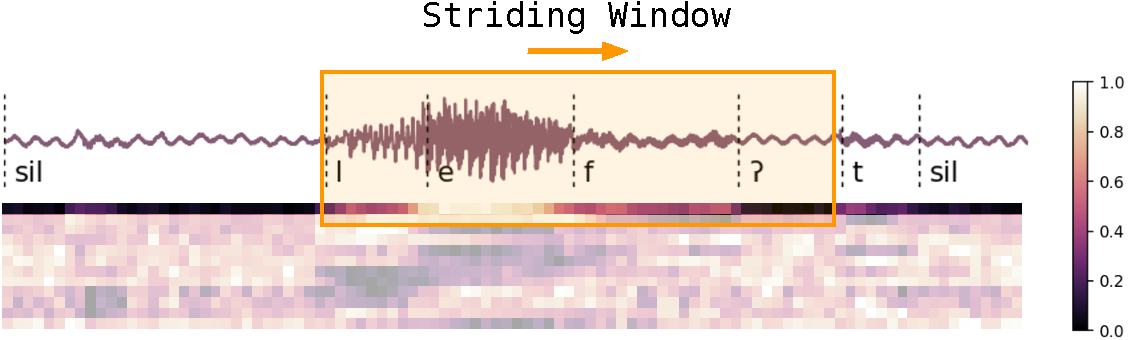
\includegraphics[width=0.65\textwidth]{./3_signal/figs/signal_onset_window.pdf}
  \caption{Striding window of length \SI{500}{\milli\second} used for energy calculation in the keyword onset detection.}
  \label{fig:signal_onset_window}
\end{figure}
\FloatBarrier
\noindent
A showcase on the performance of both energy onset detection methods is provided in \rfig{signal_onset_showcase}.
\begin{figure}[!ht]
  \centering
    \subfigure[left]{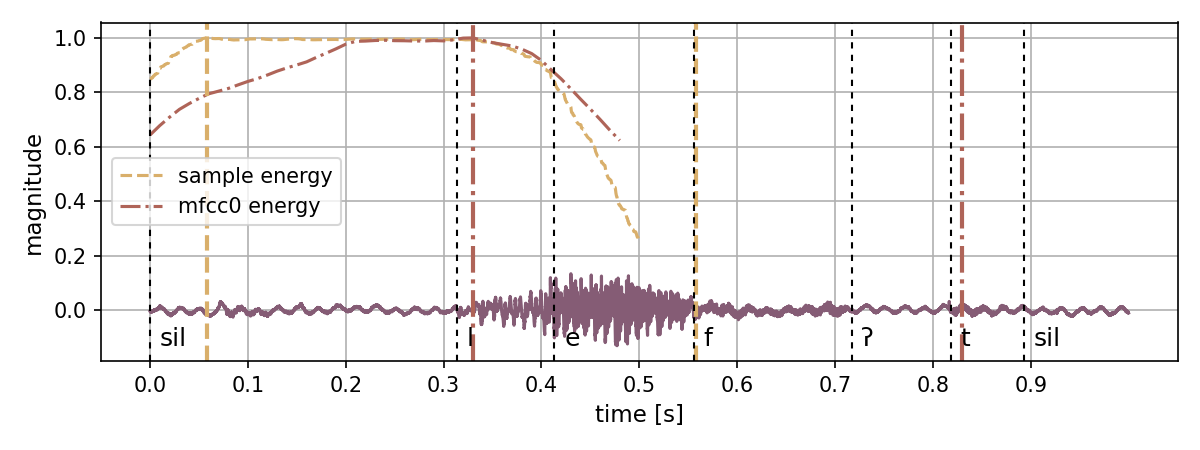
\includegraphics[width=0.45\textwidth]{./3_signal/figs/signal_onset_showcase_left0.png}}
    \quad
    \subfigure[right]{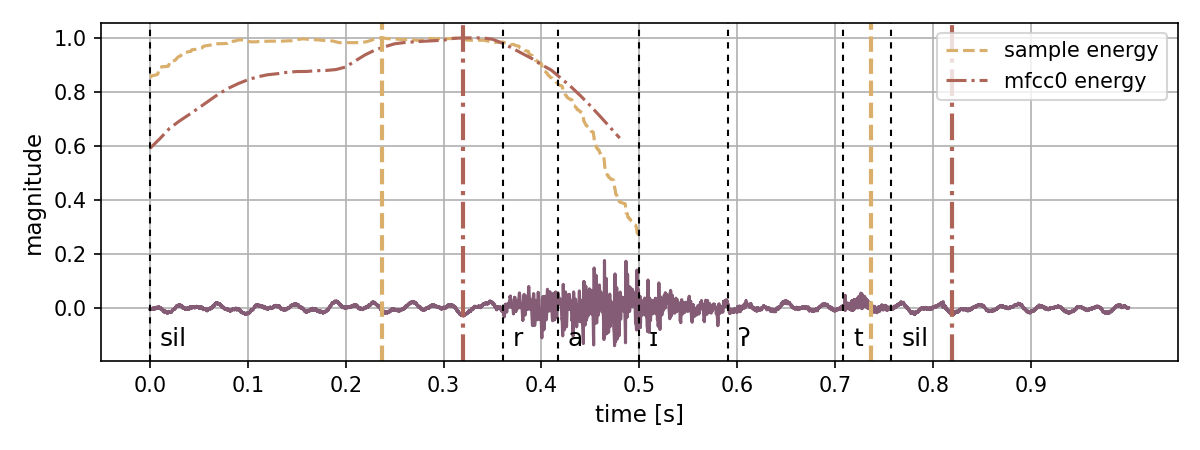
\includegraphics[width=0.45\textwidth]{./3_signal/figs/signal_onset_showcase_right0.png}}
    \subfigure[up]{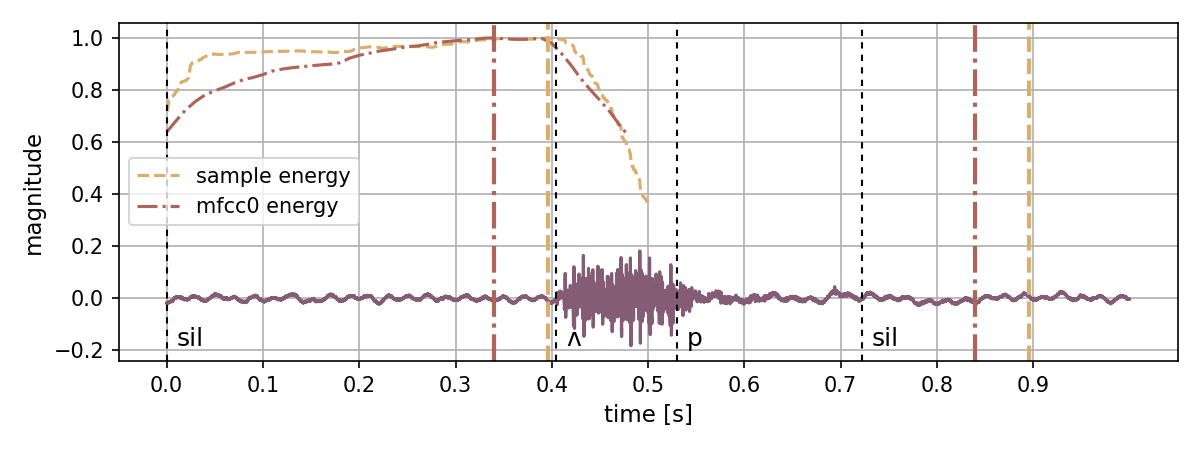
\includegraphics[width=0.45\textwidth]{./3_signal/figs/signal_onset_showcase_up0.png}}
    \quad
    \subfigure[down]{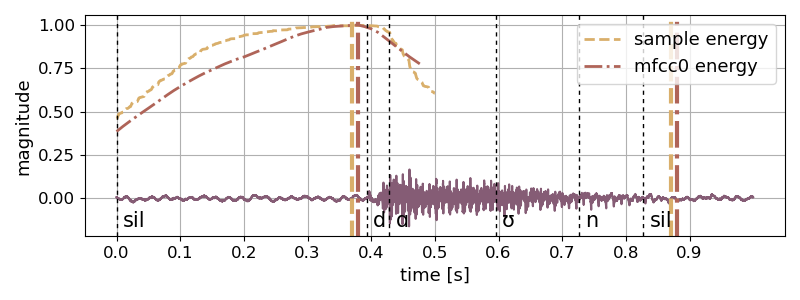
\includegraphics[width=0.45\textwidth]{./3_signal/figs/signal_onset_showcase_down0.png}}
    \subfigure[go]{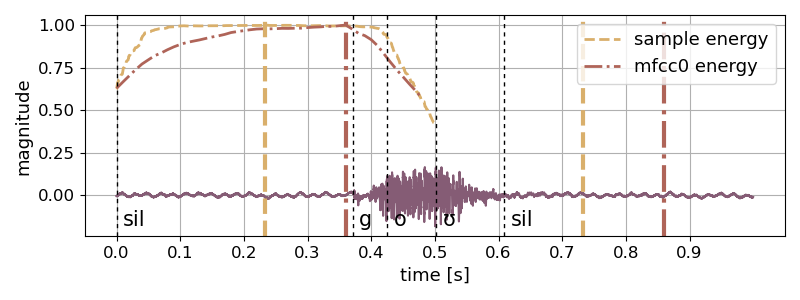
\includegraphics[width=0.45\textwidth]{./3_signal/figs/signal_onset_showcase_go0.png}}
  \caption{Onsets (vertical colored lines) obtained from the maximum of either the sample energy or first MFCC coefficient energy method with an analytic window length of \SI{500}{\milli\second}.}
  \label{fig:signal_onset_showcase}
\end{figure}
\FloatBarrier
\noindent
It can be observed that the MFCC onset method achieves better results especially for the \enquote{left} example, where a little noise peak shifts the sample energy onset too far to the left so that the analytic window at this onset position does not capture the whole word.
Note that the dataset extraction in the experiments in \rsec{exp} applies the MFCC onset method for all CNN models and the sample energy method for the Wavenet model.


% --
% keyword onset detection

\subsection{Online Onset Detection}\label{sec:signal_onset_online}
The online onset detection evaluates consecutive input chunks from online speech signals that are stored, for instance, in an data buffer.
Further, from each of the those input chunks the energy level is computed and compared with an energy threshold that indicates the presence of an onset.
It is not the purpose to detect keyword onsets by its correct starting time but to signalize whether a signal with sufficient energy is available for a potential keyword classification.
Mathematically the onset $o(\bm{x}) \in \{0, 1\}$ of an input chunk $\bm{x} \in \R^n$ from a microphone input stream can be obtained by
\begin{equation}
  o(\bm{x}) = 
  \begin{cases}
    1, & \text{if } \frac{1}{n} \bm{x}^T \bm{x} > \alpha\\
    0, & \text{otherwise} 
  \end{cases},
\end{equation}
where the output value of $1$ represents the presence of an onset, $n$ is the total sample number of the input chunk, and $\alpha$ the energy threshold.
The energy threshold should be adjustable to the user's microphone and amplifier setup. 
This can be done, for instance, in the option menu of the video game, as described in \rsec{game_design_menu}.